\documentclass{article}
\usepackage{amssymb,amsmath,amsthm}
\usepackage[hidelinks]{hyperref}
\usepackage{amssymb}
\usepackage{tikz}
\usepackage{tcolorbox}
\usepackage{graphicx}
\usepackage{marginnote}
\usepackage{svg}
\usepackage{braket}
\usepackage{tikz}
\usepackage{pgfplots}
\usepackage[italian]{babel}
\usepackage[margin=3.5cm]{geometry}
\newtheorem{theorem}{Theorem}
\usepackage{mathtools}
\usepackage{algorithm}
\usepackage{algpseudocode}
\usepackage{float}
\usepackage{mathtools}
\usetikzlibrary{arrows.meta}

\begin{document}

%%%%%%%%%%%%%%%%%%%%%% TITLE PAGE %%%%%%%%%%%%%%%%%%%%%%%
\title{Report on the Adaptive Hedge Algorithm}
\author{Gabriele Favazzi Mollica}
\maketitle
%%%%%%%%%%%%%%%%%%%%%%%%%%%%%%%%%%%%%%%%%%%%%%%%%%%%%%%%%%

\section{Introduction}
\paragraph{Prediction with Expert Advice}
The problem of prediction with expert advice is formulated as follows: 
an agent has to make a decision among $K$ experts at every round $t=1,2,\ldots,T$.
At every round an agent observes a loss vector $\ell_t \in [0,1]^K$ and has to choose a distribution $p_t$ over the experts.
The loss of the agent at round $t$ is then given by $p_t \cdot \ell_t$. The goal of the agent is to learn the correct distribution
that minimizes the cumulative regret over $T$ rounds, defined as: $ \sum_{t=1}^T (p_t \cdot \ell_t) - \min_{k=1,\ldots,K} \sum_{t=1}^T \ell_{t,k} $.
The most common algorithm to solve this problem is the Hedge algorithm, that manages to minimize the regret 
by updating the distribution $p_t$ at every round using the following rule: $p_{t+1,k} \leftarrow p_{t,k} \cdot e^{-\eta \ell_{t,k}}$, 
where $\eta$ is a learning rate parameter that controls how much the algorithm updates its distribution based on the observed losses.
The choice of the learning rate $\eta$ is crucial for the performance of the algorithm:
if $\eta$ is too small, the algorithm will be too slow to adapt to the losses and will have a high regret; if $\eta$ is too large, the algorithm will be too sensitive to the observed losses and will also have a high regret.
Compared to the classical Gradient Descent algorithm, Hedge is a multiplicative update algorithm (also known as Exponentiated Gradient), 
since it updates the distribution $p_t$ by multiplying the previous distribution with an exponential factor, while
Gradient Descent updates a point by adding a gradient step to the previous distribution.
Can be proven there exists an optimal learning rate $\eta^* = \sqrt{\frac{2\log K}{T}}$ that achieves the best possible regret bound for Hedge in the worst case, 
which is $O(\sqrt{T \log K})$ as $T$ and $K$ grow. 
For easier instances, this regret bound is too loose: previous articles already showed that, if other information are known (like the optimal cumulative loss $L_T^*$),
the regret bound can be improved to $O(\sqrt{L_T^* \log K})$. This regret bound still converges to the theoretical optimal bound showed before as $T$ and $K$ grow.

\paragraph{AdaHedge Description}
The main contribution of \cite{ADA_HEDGE} is to show that AdaHedge, an adaptive version of the Hedge algorithm, 
can adaptively adjust its learning rate $\eta$ based on the observed losses, without any prior knowledge of $T$ or $L_T^*$, 
and still achieve the optimal regret bound in the worst case, while improving it in easier instances.
The main idea behind AdaHedge is to divide the time horizon into segments,
and iteratively compute the cumulative mixability gap $\Delta$ for that segment, 
which is a measure of the gap between the expected loss of the algorithm and the logarithmic mixable loss.
More informally, $\Delta$ quantifies how difficult the current segment is for the algorithm: 
if $\Delta$ is small, it means that the algorithm is performing well and can continue to use the same learning rate; 
if $\Delta$ is large, it means that the algorithm is struggling and needs to adjust its learning rate to better adapt to the current segment.
In particular, when $\Delta$ exceeds a certain budget $b$, the algorithm starts a new segment by decreasing the learning rate $\eta$ and
resetting the learned weights and $\Delta$.
The great advantage of this approach is that adaHedge's regret doesn't depend on the time steps $T$ 
but on the number of segments started (for Lemma 4 in \cite{ADA_HEDGE}).
For Lemma 9 in \cite{ADA_HEDGE}, in case of stochastic losses, 
the number of segments is bounded by a quantity that doesn't depend on $T$. Then the regret is $O(K + \log(\frac{1}{\delta})) = O(1)$ with probability 
at least $1-\delta$, improving the original $O(\sqrt{T \log K})$ bound for Hedge.
However, in the worst case (i.e. the adversarial setting), the number of segments can be as large as $O(\sqrt{T \log K})$, 
and the regret is $O(\sqrt{T \log K})$ as well, matching the original bound for Hedge.

\section{Experiments}
In order to empirically evaluate the performance of AdaHedge compared to Hedge with different learning rates, 
I implemented both algorithms in Python and ran them on synthetic data.
Given $\eta^*$ the optimal learning rate in the worst case scenario, I decided to run Hedge with learning rates $\{\eta^*, 10\eta^*, 1000\eta^*  \}$. 
The second one should be a reasonable learning rate for the tests while
the third one is so large that it acts as Follow the Leader (FTL) strategy, at every round putting all the weight on the expert with the lowest cumulative loss so far,
which should lead to a very fast adaptation to the losses of the experts, but, in theory, also to a very high regret in case of adversarial losses.
The initial learning rate for AdaHedge is set to $\eta_0 = 1.0$ and $\phi = 2.0$ as suggested in \cite{ADA_HEDGE}.
The three settings I considered are:
\begin{itemize}
    \item \textbf{Stochastic setting}: the losses of the experts are generated from a fixed distribution, with one expert having a lower expected loss than the others.
    In particular the best expert has a loss of 1 with probability 0.3 while the other experts have a loss of 1 with probability 0.5.
    \item \textbf{Adversarial setting}: at every round, the best expert (with $loss=0$) is randomly chosen among the experts; the other experts have a loss of 1.
    \item \textbf{Low gap setting}: similar to the stochastic setting, but the best expert has a loss of 1 with probability $0.5 - \epsilon$ while 
    the other experts have a loss of 1 with probability $0.5$.
    \item \textbf{Exponential segment setting}: the number of rounds is divided into segments of lengths $1, 2, 4, ..., 2^(I-1)$, and at the beginning of each segment, one expert has a lower probability of loss than the others. 
    In particular, at every segment $m_i = 2^i$ steps, one expert has probability of loss $0.5 - \epsilon$ and the others have probability of loss $0.5$.
\end{itemize}
The number of segments is $I=9$, so the total number of rounds is $T=511$, the number of experts is $K=20$ and $\epsilon = 0.1$. The results are averaged over $n\_runs=20$ iterations 
to reduce the variance of the results.
In these experiments, the cumulative regret curve is computed starting from the vector of cumulative regrets $R_t = \sum_{s=1}^t l_s \cdot w_s - \min_{k} \sum_{s=1}^t l_s^{(k)}$;
one can observe that at each round $t$ the best cumulative loss can belong to a different expert, so the cumulative regret curve can show some "jumps" when the best expert changes, especially in the exponential segment setting.
However, by averaging the cumulative regrets, results are smoother and more readable, except for the last setting curve, which is not averaged to easily show the spikes.

\subsection{Stochastic Setting}
\begin{figure}[H]
    \centering
    \begin{minipage}{0.48\textwidth}
        \centering
        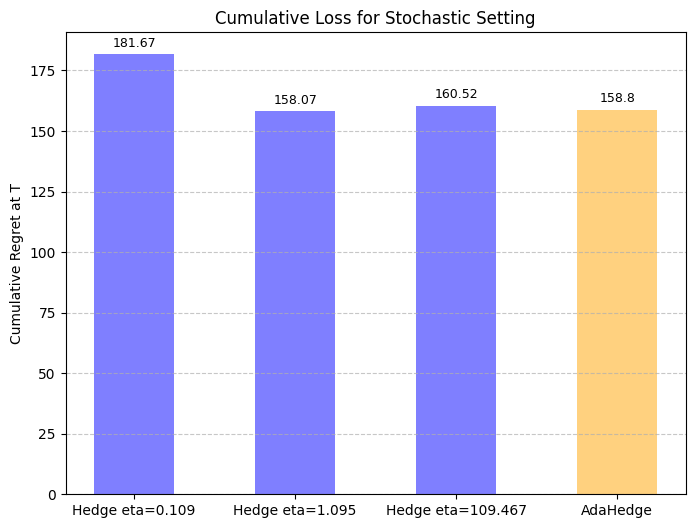
\includegraphics[width=\textwidth]{imgs/STOC_CUMLOSS.png}
        \caption{Cumulative Loss (Stochastic)}
        \label{fig:stochastic_cumloss}
    \end{minipage}
    \hfill % Inserisce spazio elastico tra le due minipage
    \begin{minipage}{0.48\textwidth}
        \centering
        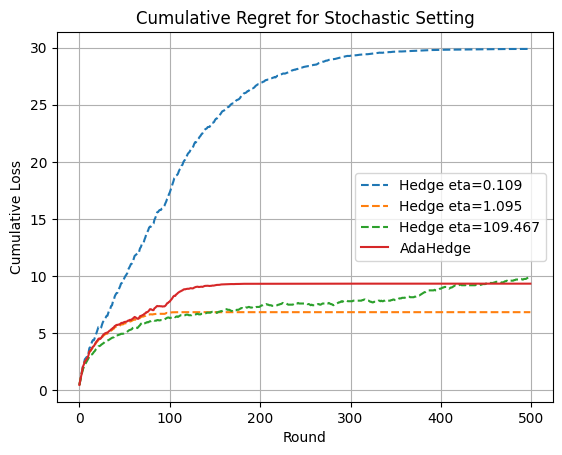
\includegraphics[width=\textwidth]{imgs/STOC_REGRET.png}
        \caption{Cumulative Regret (Stochastic)}
        \label{fig:stochastic_regret}
    \end{minipage}
\end{figure}
The results in the stochastic setting are shown in Figure \ref{fig:stochastic_cumloss} and Figure \ref{fig:stochastic_regret}.
As we expected, this is the easiest scenario, since AdaHedge started only an average of 0.23 segments and its regret is almost constant, just like FTL Hedge, 
while the other algorithms have a regret that grows with $T$.
All the algorithms show low cumulative loss, AdaHedge in particular, except for the one with the optimal learning rate $\eta^*$:
as expected, its regret is high in this easy scenario.

\subsection{Adversarial Setting}
\begin{figure}[H]
    \centering
    \begin{minipage}{0.48\textwidth}
        \centering
        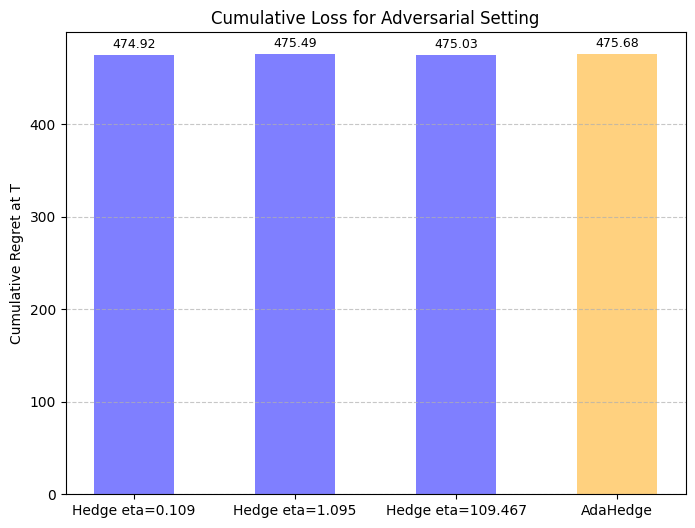
\includegraphics[width=\textwidth]{imgs/ADV_CUMLOSS.png}
        \caption{Cumulative Loss (Adversarial)}
        \label{fig:adversarial_cumloss}
    \end{minipage}
    \hfill
    \begin{minipage}{0.48\textwidth}
        \centering
        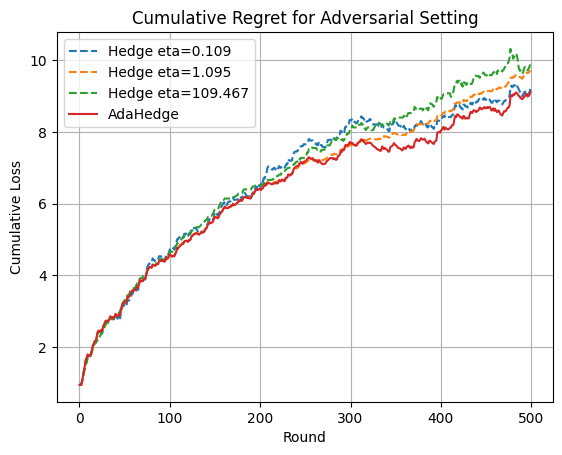
\includegraphics[width=\textwidth]{imgs/ADV_REGRET.png}
        \caption{Cumulative Regret (Adversarial)}
        \label{fig:adversarial_regret}
    \end{minipage}
\end{figure}
The results in the adversarial setting are shown in Figure \ref{fig:adversarial_cumloss} and Figure \ref{fig:adversarial_regret}.
This scenario is definitely the harder than the previous one, since all the algorithm almost had the worst possible regret, AdaHedge included.
AdaHedge started an average of $0.91$ segments, witnessing the difficulty of the scenario.
However, the algorithm with the optimal learning rate $\eta^*$ still perform slightly worse than the others.


\subsection{Low Gap Setting}
\begin{figure}[H]
    \centering
    \begin{minipage}{0.48\textwidth}
        \centering
        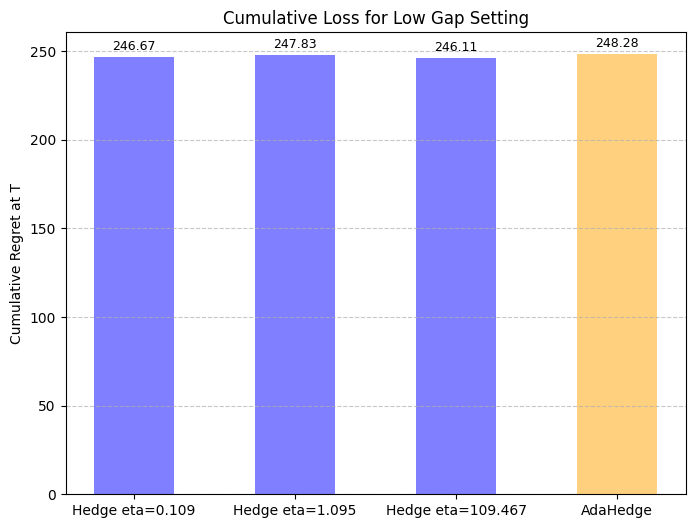
\includegraphics[width=\textwidth]{imgs/LOWGAP_CUMLOSS.png}
        \caption{Cumulative Loss (Low Gap)}
        \label{fig:lowgap_cumloss}
    \end{minipage}
    \hfill
    \begin{minipage}{0.48\textwidth}
        \centering
        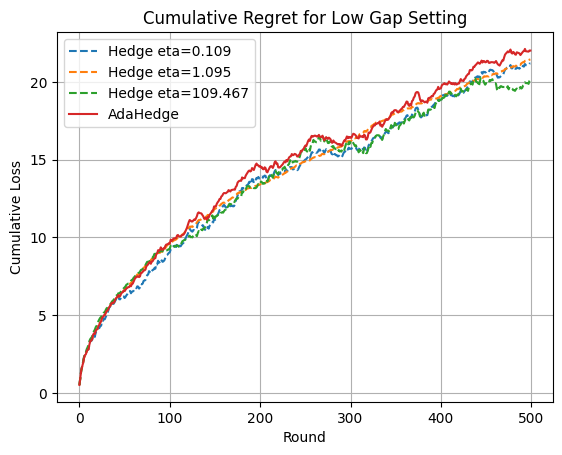
\includegraphics[width=\textwidth]{imgs/LOWGAP_REGRET.png}
        \caption{Cumulative Regret (Low Gap)}
        \label{fig:lowgap_regret}
    \end{minipage}
\end{figure}
The results in the low gap setting are shown in Figure \ref{fig:lowgap_cumloss} and Figure \ref{fig:lowgap_regret}.
Even this scenario is quite hard, since AdaHedge started an average of $2$ segments, and in general algorithms 
collected worse cumulative loss than in the stochastic setting.
The algorithms with the best cumulative loss are AdaHedge and Hedge with $\eta = 100\eta^*$;
the one with the optimal learning rate $\eta^*$ performs again worse than the others, 
showing that it requires many rounds before performing well. In this scenario the Follow-the-Leader Hedge 
performed badly, unlike the first scenario, proving that drastically changing the weights distribution leads
to a high regret when the gap between the best and the other experts is small, 
unlike AdaHedge that dynamically adjusts the learning rate and the weights distribution.


\subsection{Exponential Segment Setting}
\begin{figure}[H]
    \centering
    \begin{minipage}{0.48\textwidth}
        \centering
        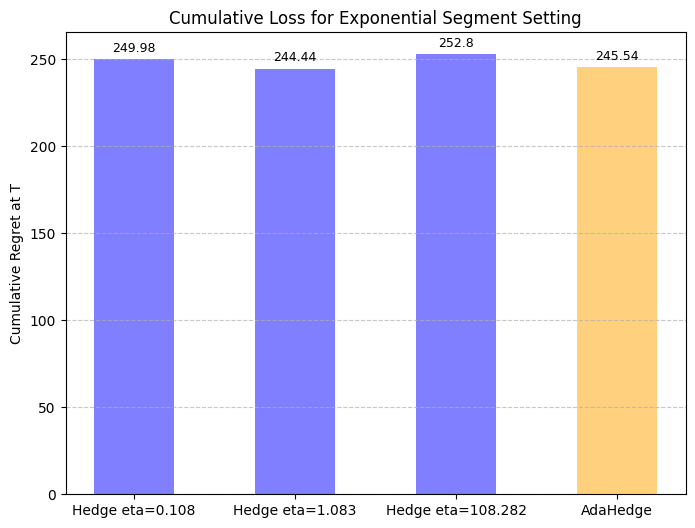
\includegraphics[width=\textwidth]{imgs/EXP_CUMLOSS.png}
        \caption{Cumulative Loss (Exponential Segment)}
        \label{fig:expseg_cumloss}
    \end{minipage}
    \hfill
    \begin{minipage}{0.48\textwidth}
        \centering
        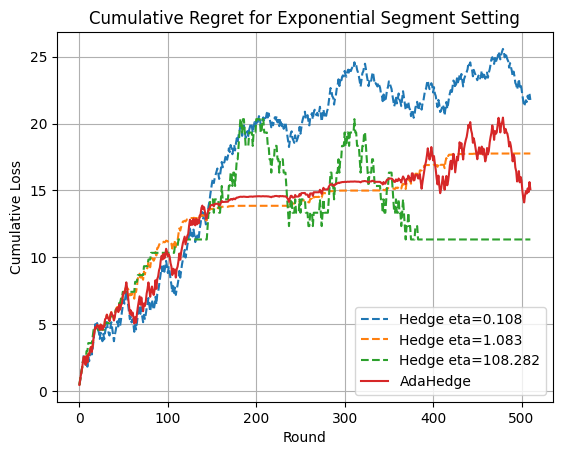
\includegraphics[width=\textwidth]{imgs/EXP_REGRET.png}
        \caption{Cumulative Regret (Exponential Segment)}
        \label{fig:expseg_regret}
    \end{minipage}
\end{figure}

This scenario is quite interesting, since it is designed to be hard for the algorithm, as the best expert changes at every segment, 
and the segments have exponentially increasing lengths, so we expect to see some stationary zones (areas in which the best expert doesn't change) as well kind of "jumps" (when the best expert changes) 
in the cumulative regret curves,
especially for the algorithms with a fixed learning rate. 
The results in the exponential segment setting are shown in Figure \ref{fig:expseg_cumloss} and Figure \ref{fig:expseg_regret}.
We can see that, as expected, the regret curves show some spikes at some points: the algorithm with the worst cumulative regret 
is still hedge with the smallest learning rate, since it is too slow to adapt to the changes in the best expert, unlike the other hedges
that are faster to adapt. In particular, the FTL Hedge perform the best since it can adapt quickly to the changes in the best expert. AdaHedge performs quite well, showing that it is able to adapt to the changes in the best expert by adjusting its learning rate and starting new segments when needed.
The number of segments started by AdaHedge is $2.78$, meaning that this scenario is even harder than the ones before, and this is also
witnessed by the high cumulative loss of all the algorithms, including AdaHedge.


%%%%%%%%%%%%%%%%%%%%%%%%%%%%%%%%%%%%%%%%%%%%%%%%%%%%%%%%%%%%%%%%%%%%%%
\begin{thebibliography}{99}
%%%%%%%%%%%%%%%%%%%%%%%%%%%%%%%%%%%%%%%%%%%%%%%%%%%%%%%%%%%%%%%%%%%%%%

\bibitem{ADA_HEDGE}
Tim van Erven, Peter Grünwald, Wouter M. Koolen, and Steven de Rooij
{\em Adaptive Hedge}, 2011, \url{https://arxiv.org/abs/1110.6416}

%%%%%%%%%%%%%%%%%%%%%%%%%%%%%%%%
\end{thebibliography}
%%%%%%%%%%%%%%%%%%%%%%%%%%%%%%%%





\end{document}
